\documentclass[10pt,twocolumn,letterpaper]{article}

\usepackage{cvpr}
\usepackage{times}
\usepackage{epsfig}
\usepackage{graphicx}
\usepackage{amsmath}
\usepackage{amssymb}
\usepackage{float}
\usepackage{listings}
\usepackage{color} %red, green, blue, yellow, cyan, magenta, black, white
\definecolor{mygreen}{RGB}{28,172,0} % color values Red, Green, Blue
\definecolor{mylilas}{RGB}{170,55,241}
\usepackage{subcaption}

% Include other packages here, before hyperref.

% If you comment hyperref and then uncomment it, you should delete
% egpaper.aux before re-running latex.  (Or just hit 'q' on the first latex
% run, let it finish, and you should be clear).
\usepackage[breaklinks=true,bookmarks=false]{hyperref}

\cvprfinalcopy % *** Uncomment this line for the final submission

\def\cvprPaperID{****} % *** Enter the CVPR Paper ID here
\def\httilde{\mbox{\tt\raisebox{-.5ex}{\symbol{126}}}}

% Pages are numbered in submission mode, and unnumbered in camera-ready
%\ifcvprfinal\pagestyle{empty}\fi
\setcounter{page}{1}
\begin{document}

%%%%%%%%% TITLE
\title{Machine Learining for Computer Vision Coursework 2\\
	Visual Categorisation by BoW (K-means) and SVM
	}

\author{David Angelov\\
MEng Electrical and Electronic Engineering \\
Imperial College London\\
{\tt\small david.angelov12@imperial.ac.uk}
% For a paper whose authors are all at the same institution,
% omit the following lines up until the closing ``}''.
% Additional authors and addresses can be added with ``\and'',
% just like the second author.
% To save space, use either the email address or home page, not both
\and
Huaqi Qiu\\
MSc Communication and Signal Processing\\
Imperial College London\\
{\tt\small h.qiu15@imperial.ac.uk}
}

\maketitle
%\thispagestyle{empty}

%%%%%%%%% BODY TEXT
\section{Question 1}

%-------------------------------------------------------------------------
%\begin{figure}[H]
%	\begin{center}
%		\includegraphics[width=0.8\linewidth]{q1_meanface}
%		\caption{Mean face}
%	\end{center}
%	\label{fig:q1_meanface}
%\end{figure}



%------------------------------------------------------------------------
\section{Question 2}

\subsection{Theory of SVM and multi-class extension}
In this coursework, we applied Support Vector Machine (SVM) as the classifier. SVM is a binary classifier based on the discriminant function

\begin{equation}
y(\boldsymbol{x}) = \boldsymbol{w^T x} + b
\label{eq:svm_linear}
\end{equation}

where $\boldsymbol{w}$ is a weight vector and $b$ is the bias. The dataset $x$ is classified to one of the two classes according to the value of $y(\boldsymbol{x})$. However, there are cases when dataset is not linearly separable, in which the Kernel Trick is required. The Kernel Trick map the data points to a higher-dimensional feature space so that the dataset is linearly separable. This process is denoted by: $\boldsymbol{x} \rightarrow \phi (\boldsymbol{x})$. Now the binary SVM function (Eq.\ref{eq:svm_linear}) becomes

\begin{equation}
y(\boldsymbol{x}) = \boldsymbol{w^T} \phi (\boldsymbol{x}) + b
\end{equation}

The SVM separate data in the Kernel transformed space by a linear decision hyperplane. The best hyperplane is found by maximizing the margin of separation. The margin is evaluated by finding the distance of the closest training point to the decision hyperplane. The optimised weighting vector $\boldsymbol{w}$ takes the form of

\begin{equation}
\boldsymbol{w} = \sum_{n=1}^{N} a_n t_n \phi(\boldsymbol{x_n})
\end{equation}

where $\boldsymbol{x_n}$ is training data vector and $t_n$ is the labels of the $n^{th}$ training data vector. Then the SVM decision function becomes

\begin{equation}
	y(\boldsymbol{x}) = \sum_{n=1}^{N} a_n t_n k(\boldsymbol{x}, \boldsymbol{x}_n)  + b
\end{equation}

where $k(\boldsymbol{x}, \boldsymbol{x}_n) $ is the Kernel function. In this course work we primarily consider the RBF kernel function, which is formulated as

\begin{equation}
 k(\boldsymbol{x}, \boldsymbol{x'}) = exp(\frac{||\boldsymbol{x} - \boldsymbol{x'}||^2}{2 \sigma^2})
\end{equation}

We considered the parameter $\sigma$ in the kernel function as the primary factor that affects the performance of RBF kernel SVM. We also considered the parameter $C$, which is an error weighting constant that penalizes the misclassification during the supervised learning and effectively controls the margin.

Since SVM is two-class classifier, we extended it in order to solve multi-class classification problems. Two methods of extension were considered:

\begin{enumerate}
	\item One versus the rest (OVR)\\
	In OVR method, we trained $M$ separate SVMs for $M$ class problem. In the training of the $m^{th}$ SVM, the $m^{th}$ class were labelled as positive class, while the rest $M-1$ classes were labelled as negative class. Upon testing a query image $\boldsymbol{x}$, the output from all $M$ SVMs were compared. The query image was classified as the $m^{th}$ image if the output of the $m^{th}$ SVM was the highest, i.e.
	\begin{equation}
		y(\boldsymbol{x}) = max_m \{ y_m(\boldsymbol{x}) \}
	\end{equation}
	
	\item One versus one (OVO)\\
	In OVO method, we trained SVMs by pairs of the classes. Each of the $M(M-1)/2$ SVMs was trained by data from a pair of two classes, labelling data points from one of the class as the positive class. In testing, the query image was tested and the output from each SVM was treated as 'vote'. The class that had the majority of votes was the class that the query image was classified to.
\end{enumerate}

\subsection{Implementation on Toy Spiral data}
In this coursework, we firstly tested the SVM theory on the Toy Spiral data, shown in Figure~\ref{fig:q2_data}. Each data point is in the form of $ [(X_n, Y_n), t_n]$, where $(X_n, Y_n)$ is 2-D Cartesian coordinates and $t_n$ is the class label of the data point. The testing data is a 2D dense grid within the range of $X_n, Y_n \in [-1.5, 1.5]$. Testing with this testing data set can visualise the decision boundaries.

\begin{figure}
	\begin{center}
		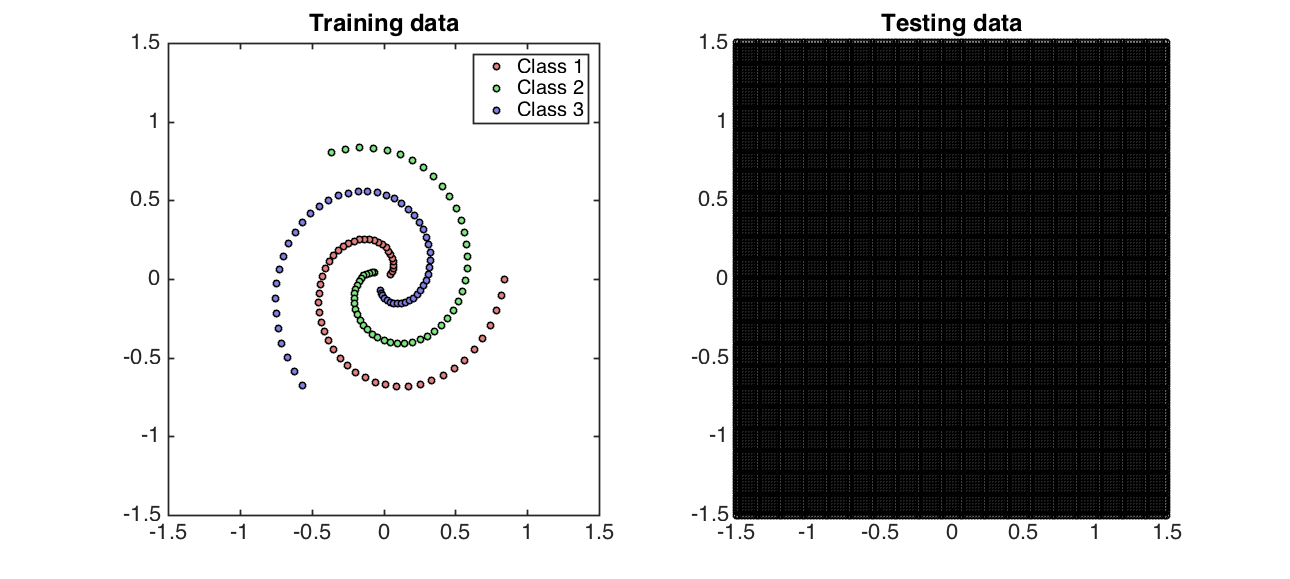
\includegraphics[width=0.8\linewidth]{q2_data}
		\caption{Toy Spiral training and testing data face}
			\label{fig:q2_data}
	\end{center}
\end{figure}

\subsection{SVM extension}
As introduced previously, we extended the binary class SVMs to multi-class SVMs by OVR and OVO. Figure~\ref{fig:q2_ovr_3} shows the classification results from each of the 3 SVMs extended by OVR method. In this Figure, red regions represents the positive class classified by the SVM. The combined classification of the 3 SVMs is shown in Figure~\ref{fig:q2_ovr}. In all demonstrations in this part of the discussion, the kernel coefficients $\sigma$ and $C$ are kept unchanged ($\sigma = 0.8$ and $C = \infty$).

\begin{figure}
	\begin{center}
		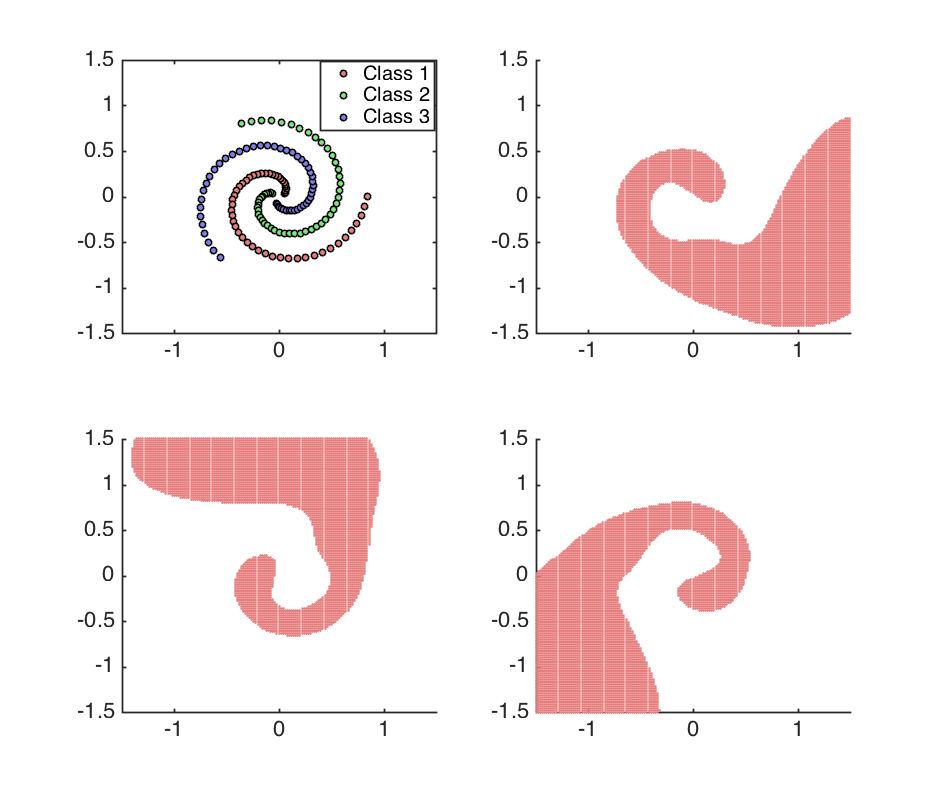
\includegraphics[width=0.8\linewidth]{q2_ovr_3}
		\caption{Result form each OVR extended SVMs}
		\label{fig:q2_ovr_3}
	\end{center}
\end{figure}

\begin{figure}
	\begin{center}
		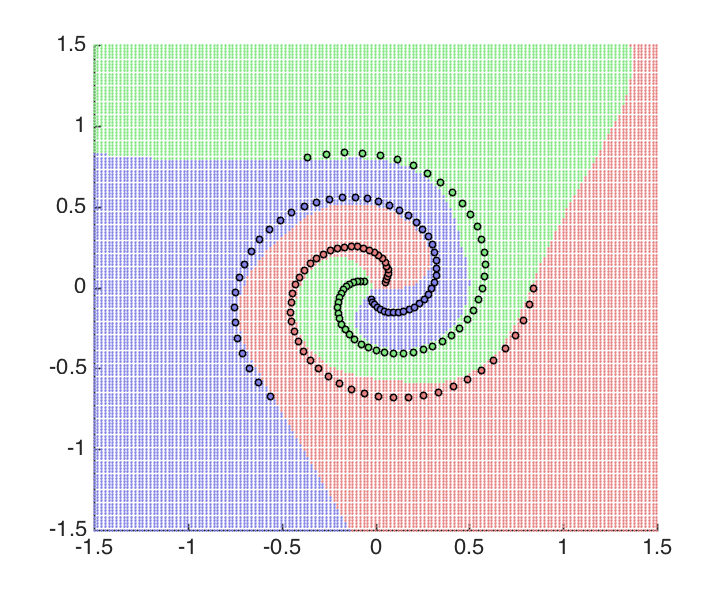
\includegraphics[width=0.8\linewidth]{q2_ovr_sig08}
		\caption{Combined result of OVR extended SVMs}
		\label{fig:q2_ovr}
	\end{center}
\end{figure}

Similarly, Figure~\ref{fig:q2_ovo_3} and~\ref{fig:q2_ovo} show the results of individual SVMs and their combination respectively. Notice that in the OVO case, the votes from all $M(M-1)$ might not have a single majority. Data points with these classification results were classified as 0 in this question, which corresponds to the 'white' area in Figure~\ref{fig:q2_ovo}. For the recognition problem of Caltech 101 data in question 4, we randomly selected class labels from all classes for these type of data points by \texttt{randi}. 

\begin{figure}
	\begin{center}
		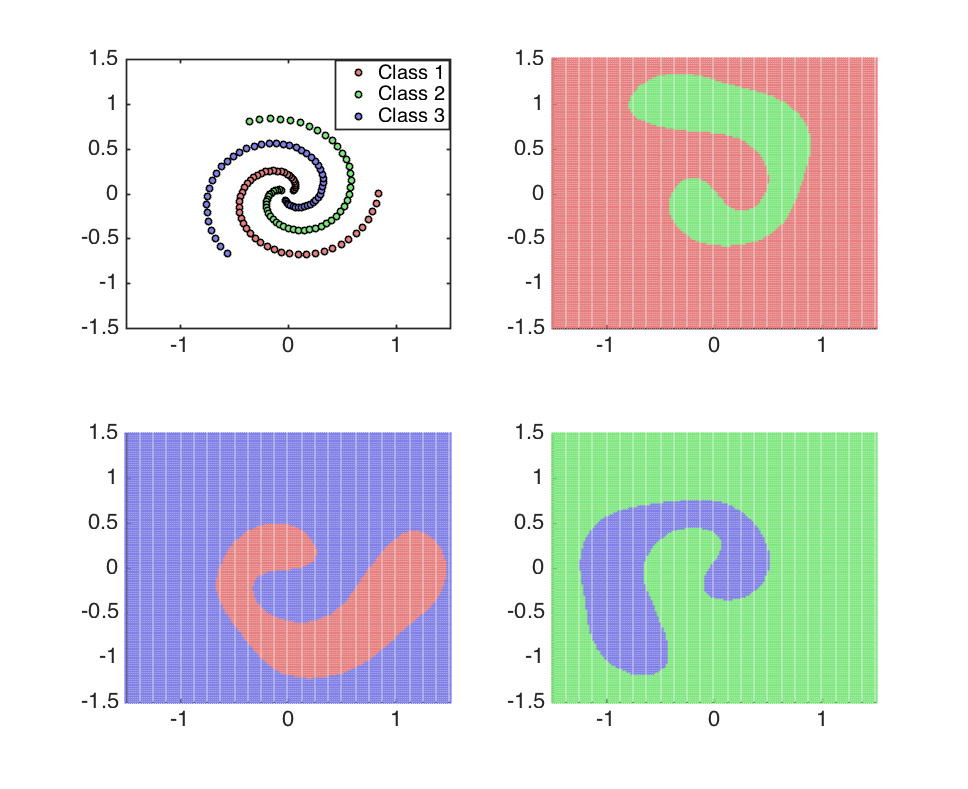
\includegraphics[width=0.8\linewidth]{q2_ovo_3}
		\caption{Result form each OVO extended SVMs}
		\label{fig:q2_ovo_3}
	\end{center}
\end{figure}

\begin{figure}
	\begin{center}
		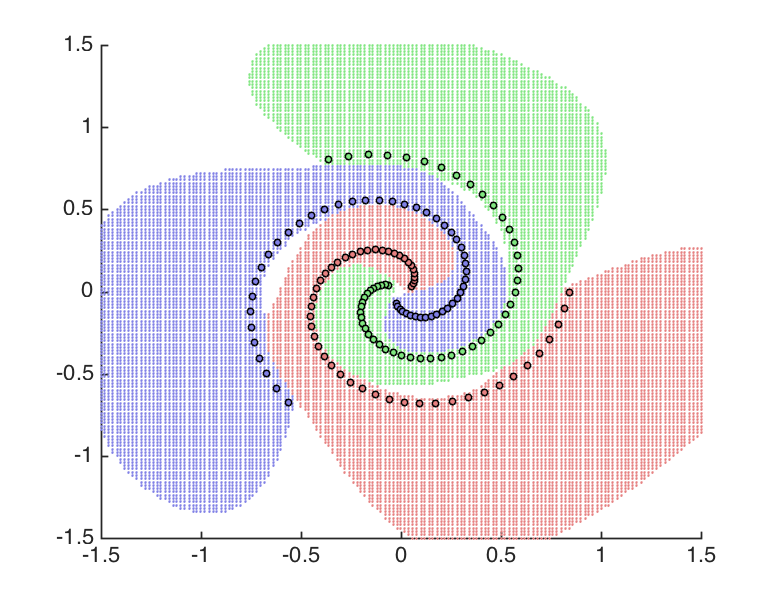
\includegraphics[width=0.8\linewidth]{q2_ovo}
		\caption{Combined result of OVO extended SVMs}
		\label{fig:q2_ovo}
	\end{center}
\end{figure}

\subsection{SVM parameters}
The kernel parameter $\sigma$ affects the generalization or complexity of the model. Simpler models could have better generalization to unseen data with the risk of underfitting. Complex models on the other hand could be overfitted to training data and results in high testing loss (i.e. lower classification accuracy). Figure (a), (b) and (c) show                                                                                              \begin{figure}

\begin{subfigure}[H]{0.3 \columnwidth}
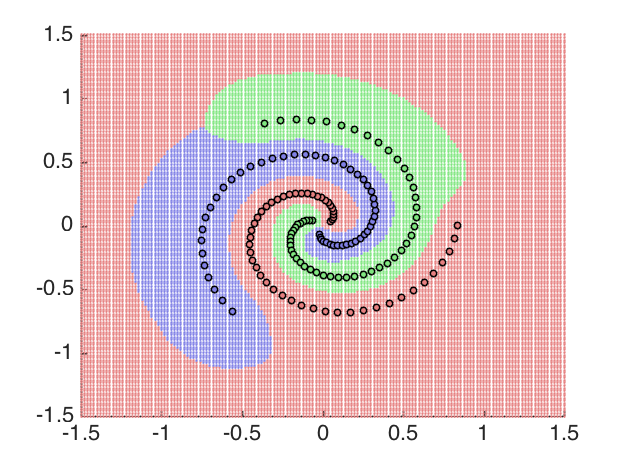
\includegraphics[width = 1\columnwidth]{q2_ovr_sig02}\hfill
\caption{$\sigma = 0.2$}
\end{subfigure}
~
\begin{subfigure}[H]{0.3 \columnwidth}
	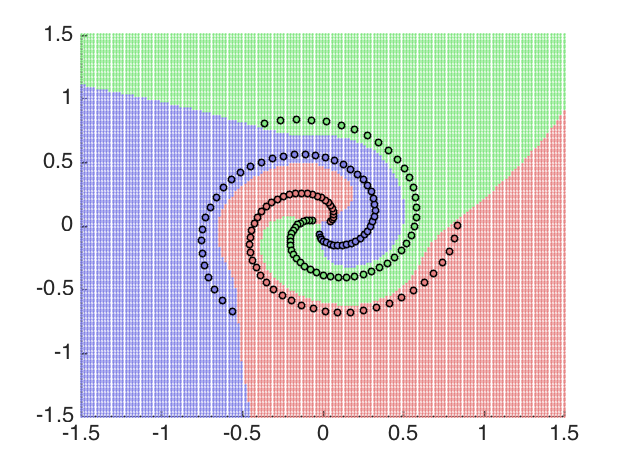
\includegraphics[width = 1\columnwidth]{q2_ovr_sig1}
	\caption{$\sigma = 1$}
\end{subfigure}
~
\begin{subfigure}[H]{0.3 \columnwidth}
	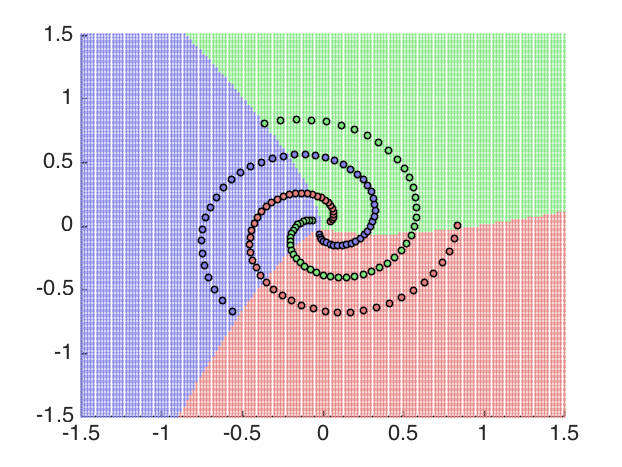
\includegraphics[width = 1\columnwidth]{q2_ovr_sig5}
	\caption{$\sigma = 5$}
\end{subfigure}

	\begin{subfigure}[H]{0.3 \columnwidth}
		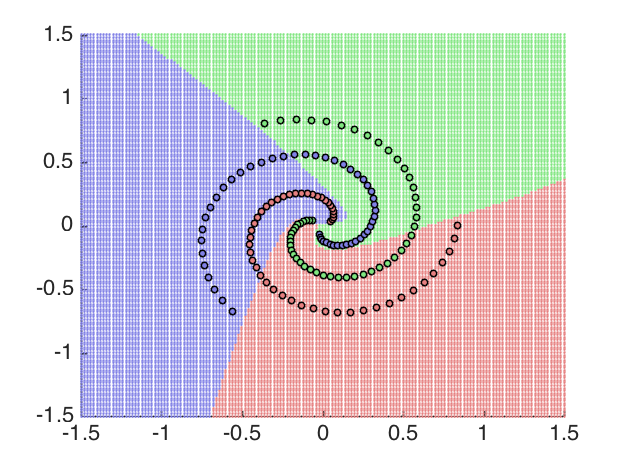
\includegraphics[width = 1\columnwidth]{q2_ovr_C1}\hfill
		\caption{$C = 1$}
	\end{subfigure}
	~
	\begin{subfigure}[H]{0.3 \columnwidth}
		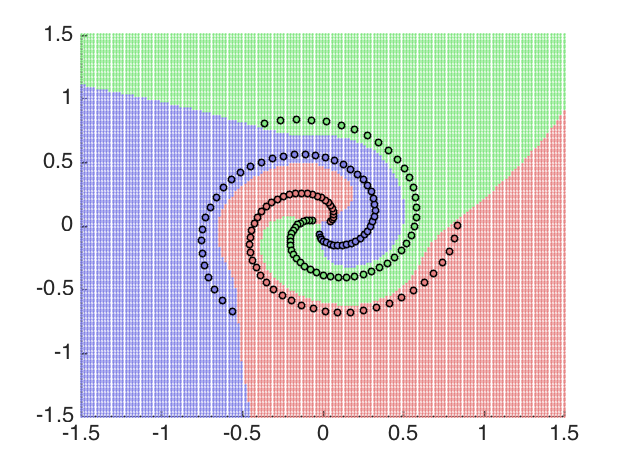
\includegraphics[width = 1\columnwidth]{q2_ovr_C1000}
		\caption{$C = 1000$}
	\end{subfigure}
	~
	\begin{subfigure}[H]{0.3 \columnwidth}
		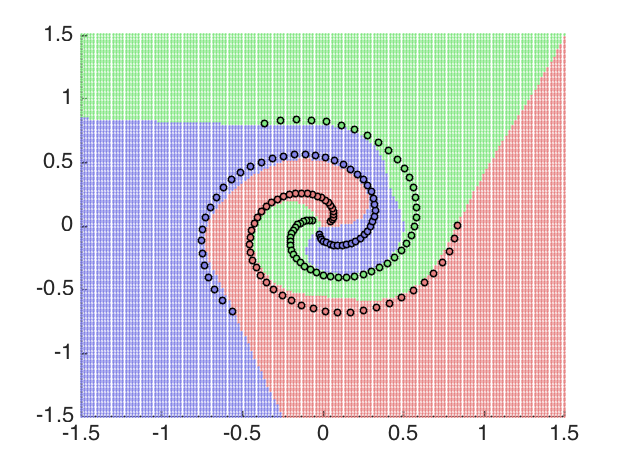
\includegraphics[width = 1\columnwidth]{q2_ovr_Cinf}
		\caption{$C = \infty$}
	\end{subfigure}
\end{figure}


\section{Question 3}




{\small
\bibliographystyle{ieee}
\bibliography{egbib}
}

\onecolumn
\appendix
\section{Appendix 1 Matlab Code}
\subsection{Init.m}
\lstinputlisting{init.m}

\section{matlab code part 2}
\lstinputlisting{init.m}



\end{document}
